\chapter{Experimental Setup} \label{ch:ExperimentalSetup}

In this chapter we present the experimental setup used to compare the two new proposals introduced in Chapter \ref{ch:NewProposals} with the current state-of-the-art. We start by briefly introducing the state-of-the-art methods in Section \ref{sec:SOTA}. Afterwards, we specify the dataset used in experimentation (Section \ref{sec:Datasets}), as well as the constraint sets (Section \ref{sec:ConstGen}) and the result evaluation method (Section \ref{sec:EvalMet}). The validation method that will be applied to the results in later chapters (Chapter \ref{ch:AnalysisResults} is discussed in Section \ref{sec:ValidtnMethod}). We also include the required configuration to replicate the experiments in Section \ref{sec:Calibration}.

\section{State-of-the-art Methods} \label{sec:SOTA}

The first adaptation of a classic clustering method for constrained clustering was proposed in \cite{wagstaff2001constrained}. It involved modifying the widely studied K-means algorithm to take into account instance-level constraints: the already known \acs{ML} and \acs{CL}. This method was named \acf{COPKM}, it introduces a modification to the assignation rule of instances to clusters of the K-means algorithm so that an instance can be assigned to a cluster only if the assignment does not violate any constraint.

In \cite{antoine2012cecm} \acf{CECM}, a variant of the Evidential c-means (\acsfont{ECM} \cite{masson2008ecm}) algorithm is proposed, within the fuzzy clustering family of methods. The particularity of this algorithm is that the membership of instances to a cluster is defined by a probabilistic belief function. This method redefines constraints from the point of view of belief functions and includes them in the cost function.

A modification of the Constrained Vector Quantization Error algorithm (\acsfont{CVQE} \cite{davidson2005clustering}) is proposed in \cite{pelleg2007k}. The \acsfont{CVQE} algorithm proved to produce high quality results, at the cost of a very high computational complexity. \acf{LCVQE} introduces a modification of the cost function of \acsfont{CVQE} to make it more intuitive and less computationally complex. The experimentation resulted in a dramatic improvement of clustering quality over both noisy and clean constraint sets.

\acf{TVClust} and \acf{RDPM} were proposed in \cite{khashabi2015clustering}. \acs{TVClust} is able to incorporate the constraints into the clustering problem by making a soft interpretation of them. The authors model the dataset and constraints in different ways, perform clustering methods on them and try to find a consensus between both interpretations. Using this model as a basis, the authors derive the \acs{RDPM} deterministic algorithm. This method can be viewed as an extension of K-means that includes side information (constraints) and has the property that the number of clusters ($k$) does not need to be specified.

\section{Datasets} \label{sec:Datasets}

For our experiments we will compare the results obtained by \acs{DILS}$_{CC}$ and \acs{SHADE}$_{CC}$ with those obtained by state-of-the-art methods and \acs{BRKGA}$_{CC}$ over twenty datasets and three constraint sets for each one of them. Most of these datasets can be found at the \href{https://sci2s.ugr.es/keel/category.php?cat=clas}{Keel-dataset repository} \cite{triguero2017keel}, though some of them have been obtained via
\href{https://scikit-learn.org/stable/datasets/index.html}{\texttt{scikit-learn} python package} \cite{scikit-learn}. We also include three artificial datasets in our analysis, namely: \textit{Circles}, \textit{Moons} and \textit{Spiral}, which can be found at \href{https://github.com/GermangUgr/DILS_CC}{GitHub}. Table \ref{tab:datasets} displays a summary of every dataset.

\begin{table}[!h]
	\centering
	%\setlength{\arrayrulewidth}{1mm}
	%\setlength{\tabcolsep}{5pt}
	%\renewcommand{\arraystretch}{1.2}
	%\resizebox{\textwidth}{!}{
	\small
	\begin{tabular}{l c c c}
		\hline
		Name & No. Instances & No. Classes & No. Features \\
		\hline
		Appendicitis & 106 & 2 & 7 \\
		Breast Cancer & 569 & 2 & 30 \\
		Bupa & 345 & 2 & 6 \\
		Circles & 300 & 2 & 2 \\
		Ecoli & 336 & 8 & 7 \\
		Glass & 214 & 6 & 9 \\
		Haberman & 306 & 2 & 3 \\
		Hayesroth & 160 & 3 & 4 \\
		Ionosphere & 351 & 2 & 33 \\
		Iris & 150 & 3 & 4 \\
		Monk2 & 432 & 2 & 6 \\
		Moons & 300 & 2 & 2 \\
		Saheart & 462 & 2 & 9 \\
		Sonar & 208 & 2 & 60 \\
		Soybean & 47 & 4 & 35 \\
		Spectfheart & 267 & 2 & 44 \\
		Spiral & 300 & 2 & 2 \\
		Tae & 151 & 3 & 5 \\
		Vowel & 990 & 11 & 13 \\
		Zoo & 101 & 7 & 16 \\
		\hline
		
	\end{tabular}%}
	\caption{Summary of datasets used for the experiments.}
	\label{tab:datasets}
\end{table}

Classification datasets are commonly used in the literature to test constrained clustering algorithms; the reason behind this is that they enable us to generate constraints with respect to the true labels (see Section \ref{sec:ConstGen}). They also facilitate an easy evaluation of the quality of the algorithm by means of measures like the Adjusted Rand Index (see Section \ref{sec:EvalMet}).

\section{Constraint Generation} \label{sec:ConstGen}

Since we have the true labels associated with each dataset, we will use the method proposed in \cite{wagstaff2001constrained} to generate artificial constraint sets. This method consists of randomly selecting two instances of a dataset, then comparing its labels, and finally setting an \acs{ML} or \acs{CL} constraint depending on whether the labels are the same or different.

We will generate, for each dataset, three different sets of constraints---$CS_{10}$, $CS_{15}$ and $CS_{20}$---that will be associated with three small percentages of the size of the dataset: 10\%, 15\% and 20\%. With $n_f$ being the fraction of the size of the dataset associated with each of these percentages, the formula $(n_f(n_f-1))/2$ tells us how many artificial constraints will be created for each constraint set; this number is equivalent to how many edges a complete graph with $n_f$ vertices would have. Table \ref{tab:constraints} shows the number of constraints of each type obtained for each dataset.

\begin{table}[!h]
	\centering
	%\setlength{\tabcolsep}{7pt}
	%\renewcommand{\arraystretch}{1}
	%\begin{adjustwidth}{-1in}{-1in}
	\resizebox{\textwidth}{!}{
		\begin{tabular}{lcc c cc c cc}
			\hline
			\multirow{2}{*}{Dataset} &
			\multicolumn{2}{c}{$CS_{10}$} && \multicolumn{2}{c}{$CS_{15}$} && \multicolumn{2}{c}{$CS_{20}$} \\
			\cline{2-3} \cline{5-6} \cline{8-9}
			& \acs{ML} & \acs{CL} && \acs{ML} & \acs{CL} && \acs{ML} & \acs{CL} \\
			\hline
			Appendicitis & 39 & 16 && 71 & 49 && 164 & 67 \\
			Breast Cancer & 876 & 720 && 1965 & 1690 && 3487 & 2954 \\
			Bupa & 323 & 272 && 699 & 627 && 1201 & 1145 \\
			Circles & 208 & 227 && 502 & 488 && 853 & 917 \\
			Ecoli & 163 & 398 && 357 & 918 && 609 & 1669 \\
			Glass & 52 & 179 && 139 & 389 && 259 & 644 \\
			Haberman & 304 & 161 && 634 & 401 && 1135 & 756 \\
			Hayesroth & 39 & 81 && 102 & 174 && 177 & 319 \\
			Ionosphere & 330 & 300 && 732 & 646 && 1299 & 1186 \\
			Iris & 26 & 79 && 82 & 171 && 136 & 299 \\
			Monk2 & 473 & 473 && 979 & 1101 && 1917 & 1824 \\
			Moons & 200 & 235 && 494 & 496 && 900 & 870 \\
			
			Saheart & 595 & 486 && 1292 & 1123 && 2330 & 1948 \\
			Sonar & 100 & 110 && 245 & 251 && 436 & 425 \\
			Soybean & 4 & 6 && 6 & 22 && 12 & 33 \\
			Spectfheart & 233 & 118 && 543 & 277 && 965 & 466 \\
			Spiral & 224 & 211 && 487 & 503 && 918 & 852 \\
			Tae & 40 & 80 && 82 & 171 && 151 & 314 \\
			Vowel & 445 & 4406 && 1026 & 10000 && 1705 & 17798 \\
			Zoo & 21 & 34 && 29 & 91 && 41 & 169 \\
			\hline
			
	\end{tabular}}
	%\end{adjustwidth}
	
	\caption{Number of constraints used in experiments.}
	\label{tab:constraints}
\end{table}

The random allocation of constraints has a potential advantage over simply using the constraints contained in an $n_f$-vertex complete graph: there is a lower probability of biasing the constraint set towards having classes with poor representation in it. Note that the greater the number of classes present in the dataset, the fewer \acs{ML} constraints obtained with the method proposed in \cite{wagstaff2001constrained}. This is because the probability of randomly choosing two individuals from the same class decreases as the number of classes present in the dataset increases. Figure \ref{fig:IrisConst} displays a visual representation of the constraint sets generated for the Iris dataset.

\begin{figure}[bth]
	\myfloatalign
	\subfloat[$CS_{10}$ \acs{ML} constraints.]
	{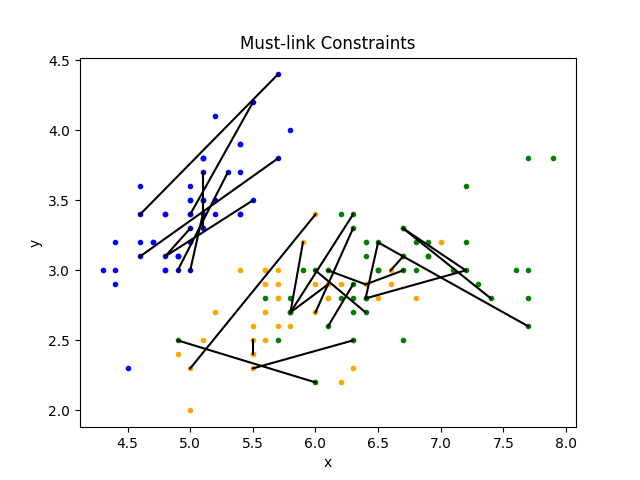
\includegraphics[width=0.45\linewidth]{gfx/ExpSetup/ML10.png}} 
	\subfloat[$CS_{10}$ \acs{CL} constraints.]
	{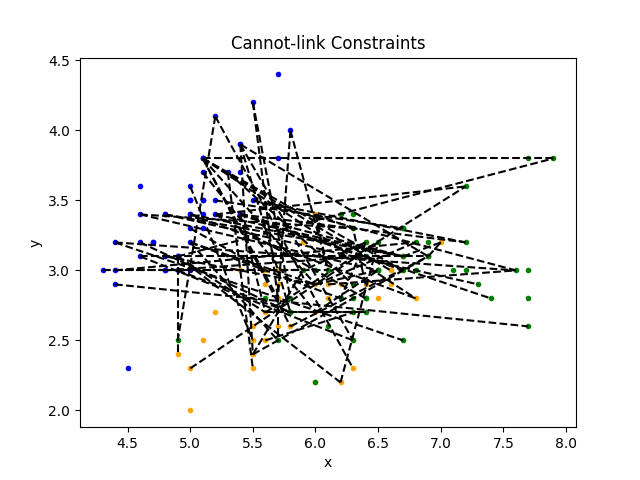
\includegraphics[width=0.45\linewidth]{gfx/ExpSetup/CL10.png}} \quad
	\subfloat[$CS_{15}$ \acs{ML} constraints.]
	{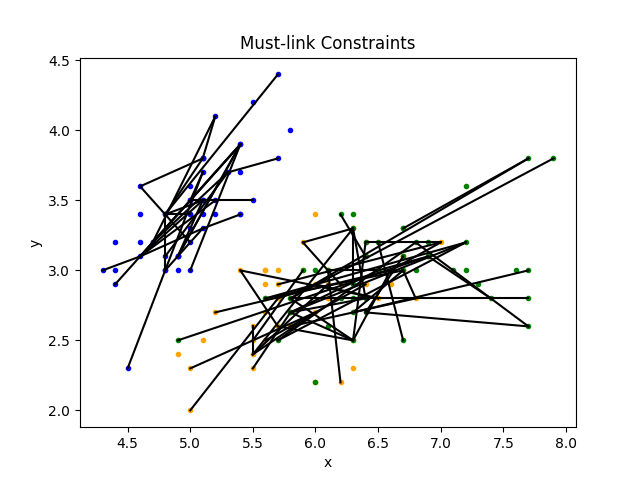
\includegraphics[width=0.45\linewidth]{gfx/ExpSetup/ML15.png}} 
	\subfloat[$CS_{15}$ \acs{CL} constraints.]
	{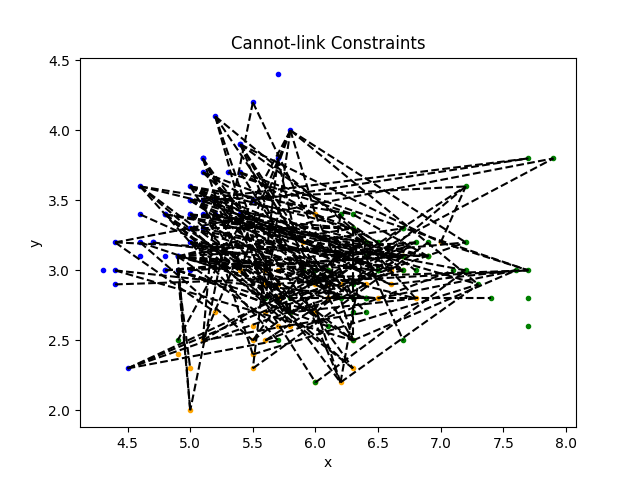
\includegraphics[width=0.45\linewidth]{gfx/ExpSetup/CL15.png}} \quad
	\subfloat[$CS_{20}$ \acs{ML} constraints.]
	{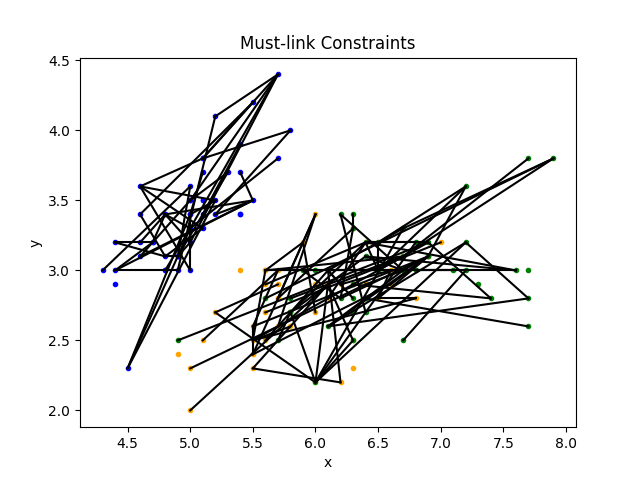
\includegraphics[width=0.45\linewidth]{gfx/ExpSetup/ML20.png}} 
	\subfloat[$CS_{20}$ \acs{CL} constraints.]
	{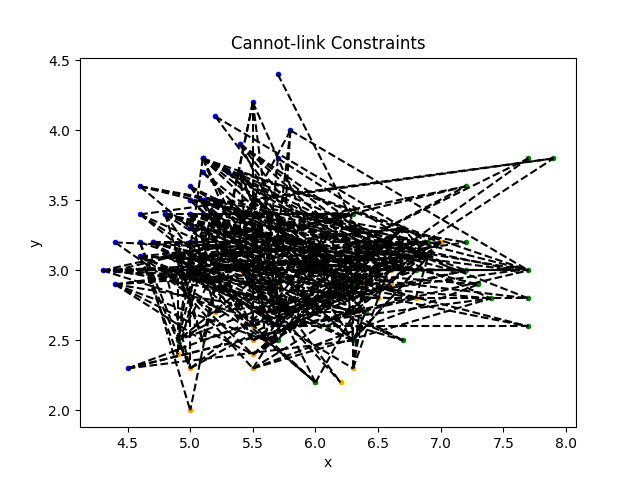
\includegraphics[width=0.45\linewidth]{gfx/ExpSetup/CL20.png}} 
	\caption{Visual representation of the three constraint sets over the Iris dataset.}
	\label{fig:IrisConst}
\end{figure}

\section{Evaluation Method} \label{sec:EvalMet}

Since we have the true labels associated with each of the datasets, we can use them to evaluate the results provided by each method. We will use the \acf{ARI} to measure the accuracy of the predictions resulting from each method we test \cite{hubert1985comparing}. The basic Rand Index computes the degree of agreement between two partitions $C_1$ and $C_2$ of a given dataset $X$. $C_1$ and $C_2$ are viewed as collections of $n(n - 1)/2$ pairwise decisions \cite{rand1971objective}.

For each pair of instances $x_i$ and $x_j$ in $X$, a partition assigns them to the same cluster or to different clusters. We take $a$ as the number of pairings where $x_i$ is in the same cluster as $x_j$ in both $C_1$ and $C_2$, and $b$ as the opposite event ($x_i$ and $x_j$ are in different clusters in $C_1$ and $C_2$). Then, the degree of similarity between $C_1$ and $C_2$ is calculated as in Equation \eqref{eq15}.

\begin{equation}
\text{Rand}(C_1, C_2) = \frac{a + b}{n(n - 1)/2}.
\label{eq15}
\end{equation}

The \acs{ARI} is a corrected-for-chance version of the Rand Index. This correction uses the expected similarity of all comparisons between clusterings specified by a random model to set up a baseline. The \acs{ARI} is computed as in Equation \eqref{eq16}.

\begin{equation}
\text{ARI}(C_1, C_2) = \frac{\text{Rand}(C_1, C_2) - \text{Expected Index}}{\text{Maximum Index} - \text{Expected Index}}\;\;,
\label{eq16}
\end{equation}

\noindent where Maximum Index is expected to be 1 and Expected Index is the already mentioned expected degree of similarity with a random model. It is easy to see that $\text{ARI}(C_1, C_2) \in [-1,1]$, such that an \acs{ARI} value close to 1 means a high degree of agreement between $C_1$ and $C_2$, a positive value close to 0 means no agreement and a value smaller that 0 means that the $\text{Rand}(C_1, C_2)$ is less than expected when comparing with random partitions. To summarize, the higher the \acs{ARI}, the greater the degree of similarity between $C_1$ and $C_2$. For more details on \acs{ARI} see \cite{hubert1985comparing}.

Our objective is to quantify the quality of the solutions obtained as a result of the methods presented in this work. To accomplish this task we just set one of the two partitions given to compute \acs{ARI} as the ground truth labels.

\section{Validation of Results} \label{sec:ValidtnMethod}

In order to validate the results which will be presented in Chapter \ref{ch:ExperimentalResults} we will use Bayesian statistical tests, instead of the classic \acf{NHST}. In \cite{benavoli2017time} we find an in-depth analysis of the disadvantages of \acs{NHST}, and a new model is proposed for carrying out comparisons researchers are interested in. \textit{"In a nutshell: \acs{NHST} do not answer the question we ask"}. To put it clear, the disadvantages of the \acs{NHST} that the authors highlight in \cite{benavoli2017time} are based on the trap of black-and-white thinking, this is: To reject, or not to reject?

To start with, \acs{NHST} do not provide us with the probabilities associated to the analyzed hypotheses, and therefore it is not possible to answer the question: What is the probability that two methods are different? Another pitfall of \acs{NHST} is that, with a sufficiently large number of observations, it is possible to reject almost any hypothesis. This is because the p-value does not allow us to separate between the effective size and the sample size, which is established by the researcher.

Also, \acs{NHST} do not provide information about the magnitude of the effects and the uncertainty of its estimate. As a consequence, \acs{NHST} may reject hypotheses despite very small effects, or even if there is significant uncertainty in the magnitude of the effects.

Furthermore, and this is a situation that all researchers have faced, \acs{NHST} do not provide any information about the null hypothesis! That is: What can we conclude when \acs{NHST} do not reject the null hypothesis? We can not infer anything since \acs{NHST} can not provide evidence in its favor.

Finally, there are two other problems that researchers face when performing \acs{NHST}. The first one is the choice of the significance level $\alpha$, for which there are no objective guidelines despite being critical to the test results. The second one is the need to previously formalize the intentions of the sampling of the results, which are usually fixed a posteriori; this could lead to a misreading of said results.

As shown in \cite{benavoli2017time}, most of these problems can be avoided by using Bayesian tests instead of \acs{NHST}. In particular we will use the Bayesian sign test, which is the Bayesian version of the frequentist non-parametric sign test. To make use of it we will employ the R package \texttt{rNPBST}, whose documentation and guide can be found in \cite{carrasco2017rnpbst}.

We will use the Bayesian sign test to validate our results, which is based on obtaining the statistical distribution of a certain parameter $\rho$ according to the difference between the results, under the assumption that said distribution is a Dirichlet distribution. To get the distribution of $\rho$ we count the number of times that $A - B < 0$, the number of times where there are no significant differences, and the number of times that $A - B > 0$. In order to identify cases where there are no significant differences, we define the region of practical equivalence (rope) $[r_\text{min}, r_\text{max}]$, so that $P(A \approx B) = P(\rho \in \text{rope})$. Using these results we calculate the weights of the Dirichlet distribution and sample it to get a set of triplets with the following form: \\

\noindent\resizebox{\textwidth}{!}{$[P(\rho < r_\text{min}) = P(A - B < 0),\;\; P(\rho \in \text{rope}),\;\; P(\rho > r_\text{max}) = P(A - B > 0)]$}

\section{Calibration} \label{sec:Calibration}

Table \ref{tab:paramsSHADE} shows a summary of the parameter setup used for both \acs{BRKGA}$_{CC}$ and \acs{SHADE}$_{CC}$ algorithms. Since both of these methods are nature-inspired population-based optimization schemes it is worth going in depth in they performance similarities and differences. All parameters have been set with the aid to achieve a fair comparison, which will be later presented in Chapter \ref{ch:ExperimentalResults}.

\begin{table}[!h]
	\centering
	\setlength{\tabcolsep}{7pt}
	\renewcommand{\arraystretch}{1.4}
	%\begin{adjustwidth}{-1in}{-1in}
	%\resizebox{\textwidth}{!}{
		\begin{tabular}{c l cc}
			\hline
			Parameter & Meaning & \acs{BRKGA}$_{CC}$ & \acs{SHADE}$_{CC}$ \\
			\hline
			$|P|$ & Population size & 100 & 100 \\
			Evals & Fitness function evaluations & 300000 & 300000 \\
			$P_e$ & \makecell[l]{Size of the elite set in \\ population} & $0.2 * |P|$ & $0.25 * |P|$ \\
			$P_m$ & \makecell[l]{Number of mutants to be \\ introduced in the population in \\ each generation} & $0.2 * |P|$ & - \\
			$p_\text{inherit}$ & \makecell[l]{Probability that a feature is \\ inherited  from an elite parent} & $50\%$ & - \\
			$k$ & \makecell[l]{Output partition number of \\ clusters} & \multicolumn{2}{m{4cm}}{No. Classes (Table \ref{tab:datasets})} \\
			\hline
			
	\end{tabular}%}
	%\end{adjustwidth}
	
	\caption{Parameter setup used for \acs{BRKGA}$_{CC}$ and \acs{SHADE}$_{CC}$.}
	\label{tab:paramsSHADE}
\end{table}

\newpage

Table \ref{tab:paramsDILS} shows a summary of the parameter setup used for the \acs{DILS}$_{CC}$ method. All parameters related to the new proposals---\acs{SHADE}$_{CC}$ and \acs{DILS}$_{CC}$---have been set experimentally, no theoretical or in-depth experimental analysis have been carried out to find an optimal tune for them.

\begin{table}[!h]
	\centering
	\setlength{\tabcolsep}{7pt}
	\renewcommand{\arraystretch}{1.4}
	%\begin{adjustwidth}{-1in}{-1in}
	\resizebox{\textwidth}{!}{
		\begin{tabular}{c l c}
			\hline
			Parameter & Meaning & Value \\
			\hline
			Evals & Fitness function evaluations & 300000 \\
			$p_s$ & \makecell[l]{Segment size for the mutation \\ operator} & $0.3 \times n$ \\
			$p_m$ & \makecell[l]{Maximum number of neighbors \\ generated in each call to the \acs{LS} \\ procedure} & Evals $\times 0.01$ \\
			$p_r$ & \makecell[l]{Probability that a feature is selected \\ from $m_b$ for recombination} & $0.3$ \\
			$\xi$ & Reinitialization method tolerance & $0.2$ \\
			$k$ & Output partition number of clusters & No. Classes (Table \ref{tab:datasets}) \\
			\hline
			
	\end{tabular}}
	%\end{adjustwidth}
	
	\caption{Parameter setup used for \acs{DILS}$_{CC}$.}
	\label{tab:paramsDILS}
\end{table}

In all three cases---\acs{BRKGA}$_{CC}$, \acs{SHADE}$_{CC}$ and \acs{DILS}$_{CC}$---the stopping criterion is given by the number of evaluations of the fitness function, which at most will be 300000. To compare with the state-of-the-art methods mentioned in Section \ref{sec:SOTA} we will use the parameters setup shown in Table \ref{tab:paramsSOTA}.

\clearpage

\begin{table}[!h]
	\centering
	\setlength{\tabcolsep}{7pt}
	\renewcommand{\arraystretch}{1.4}
	%\begin{adjustwidth}{-1in}{-1in}
	\resizebox{\textwidth}{!}{
		\begin{tabular}{>{\centering\arraybackslash}c m{5cm} c}
			\hline
			Common Parameters & Meaning & Value \\
			\hline
			\texttt{max\_iter} & Maximum number of iterations & 300 \\
			$k$ & Output partition number of clusters & No. Classes (Table \ref{tab:datasets}) \\
			\hline
			\hline
			Specific Parameters & \multicolumn{2}{l}{Name and Value} \\
			\hline
			\acs{COPKM} & \multicolumn{2}{l}{\texttt{tolerance} = $1 * 10^{-4}$; \texttt{init\_mode} = \texttt{``rand''}} \\
			\acs{CECM} & \multicolumn{2}{l}{$\alpha = 1$, $\rho = 100$, $\xi = 0.5$, \texttt{stop\_threshold} = $1 * 10^{-3}$, \texttt{init\_mode} = \texttt{``rand''}} \\
			\acs{LCVQE} & \multicolumn{2}{l}{\texttt{initial\_centroids} = $\emptyset$} \\
			\acs{RDPM} & \multicolumn{2}{l}{$\xi_0 = 0.1$, $\xi_\text{rate} = 1$, $\lambda$ is calculated on the basis of the mean distances in the dataset} \\
			\acs{TVClust} & \multicolumn{2}{l}{$\alpha_0 = 1.2$, \texttt{stop\_threshold} = $5*10^{-4}$} \\
			\hline
			
	\end{tabular}}
	%\end{adjustwidth}
	
	\caption{Parameter setup used for the state-of-the-art algorithms.}
	\label{tab:paramsSOTA}
\end{table}

Parameter values have been assigned following the guidelines of the original creators of the different proposals. Since the evaluation in the experimental stage makes use of a high number of datasets, tuning each parameter specifically for each dataset is not feasible. Indeed, our goal is not optimization in a case-by-case basis but instead a comparison in the most general scenario possible. Therefore, given that the purpose of this work is to draw a fair comparison between the algorithms and assess their robustness in a common environment with multiple datasets, we have not included a tuning step to maximize any particular performance metric. Equivalent results can be obtained with the parameters described above when used in the Python implementation found at \href{https://github.com/GermangUgr}{GitHub}\footnote{https://github.com/GermangUgr}.